\documentclass{standalone}

\usepackage{tikz}

\definecolor{cheddar}{HTML}{FFA300}
\definecolor{myorange}{HTML}{d93f2b}

\begin{document}
    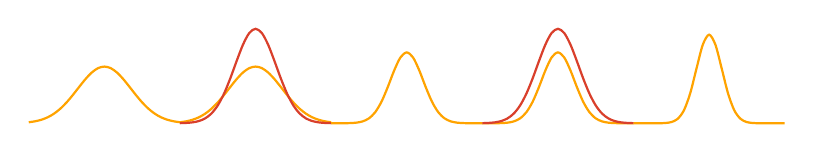
\begin{tikzpicture}[smooth, domain=-1:1,scale=0.96]

    % Assimilation 1
        %% prior 1
        \draw [thick, cheddar, variable=\x]
            plot ({\x}, {0.75 * exp(-(\x * \x)/0.25)});

        %% likelihood 1
        \begin{scope}[shift={(2, 0)}]
            \draw [thick, cheddar, variable=\x]
                plot ({\x}, {0.75 * exp(-(\x * \x)/0.25)});
            \draw [thick, myorange, variable=\x]
                plot ({\x}, {1.25 * exp(-(\x * \x)/0.15)});
        \end{scope}

        %% posterior 1
        \begin{scope}[shift={(4, 0)}]
            \draw [thick, cheddar, variable=\x]
                plot ({\x}, {1.25 * 0.75 * exp(-(\x * \x)*(1/0.15 + 1/0.25))});
        \end{scope}

    % Assimilation 2
        %% likelihood 2
        \begin{scope}[shift={(6, 0)}]
            \draw [thick, cheddar, variable=\x]
                plot ({\x}, {1.25 * 0.75 * exp(-(\x * \x)*(1/0.15 + 1/0.25))});
            \draw [thick, myorange, variable=\x]
                plot ({\x}, {1.25 * exp(-(\x * \x)/0.15)});
        \end{scope}

        %% posterior 2
        \begin{scope}[shift={(8.0, 0)}]
            \draw [thick, cheddar, variable=\x]
                plot ({\x}, {1.25 * 1.25 * 0.75 * exp(-(\x * \x)*(2/0.15 + 1/0.25))});
        \end{scope}

    \end{tikzpicture}
\end{document}